\section{Sparse coefficient growth on series--parallel networks}\label{sec:sp-growth}

The construction of \cref{sec:universality} uses unrestricted bipartite
layers. A more explicit obstruction occurs on a much narrower graph family
if the number of simplex states may grow.
For $L\ge1$, let $G_L$ have vertices $v_0,\ldots,v_L$, two arcs
$a_i,b_i:v_{i-1}\to v_i$ for each $i\in[L]$, and a bypass
$h:v_0\to v_L$. All capacities and the source--sink flow value are one.
This is a directed two-terminal series--parallel graph: first put each
pair in parallel, compose the pairs in series, and put their chain in
parallel with $h$. In a disaggregation, conservation forces
\begin{equation}\label{eq:chain-profile}
 f^j_{a_i}+f^j_{b_i}=w_j\quad(i\in[L]),\qquad
 f^j_h=\lambda_j-w_j,
 \qquad 0\le w_j\le\lambda_j.
\end{equation}
The vector $w$ is the \emph{shared branch profile}. Its total is
$\sum_jw_j=1-x_h$. Keeping only this total can lose essential
compatibility between the serial gadgets (\cref{rem:scalar-failure}).

\begin{figure}[htbp]\centering
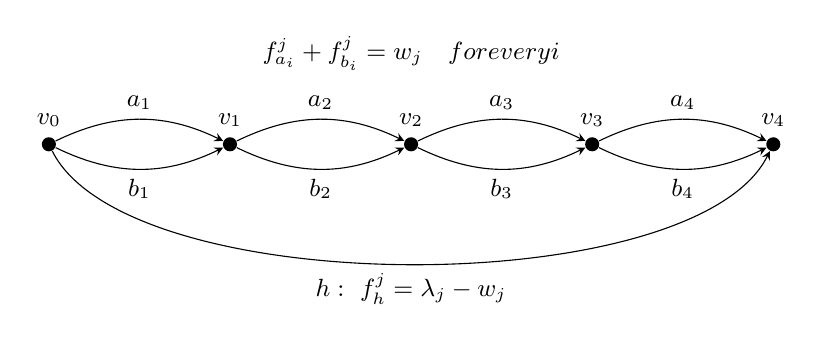
\begin{tikzpicture}[>=stealth,vertex/.style={circle,fill=black,inner sep=1.8pt},
                   every node/.style={font=\small}]
\foreach \i in {0,...,4}{
  \node[vertex,label=above:{$v_\i$}] (v\i) at (2.3*\i,0) {};
}
\foreach \i [evaluate=\i as \prev using int(\i-1)] in {1,...,4}{
  \draw[->] (v\prev) to[bend left=26] node[above] {$a_\i$} (v\i);
  \draw[->] (v\prev) to[bend right=26] node[below] {$b_\i$} (v\i);
}
\draw[->] (v0) .. controls (1,-2.0) and (8.2,-2.0) ..
  node[below] {$h:\ f_h^j=\lambda_j-w_j$} (v4);
\node at (4.6,1.15) {$f_{a_i}^j+f_{b_i}^j=w_j\quad\text{for every }i$};
\end{tikzpicture}
\caption{The flat chain $G_4$. Each serial pair carries the same statewise
branch flow $w_j$; the bypass carries the remainder. All capacities and the
source--sink flow value are one. Independent scalar totals at the four pairs
do not retain the common vector of state flows. The general $G_L$ extends
the same pattern to $L$ pairs.}\label{fig:flat-chain}
\end{figure}

\Cref{fig:flat-chain} shows the common profile on $G_4$, the graph of the
coefficient-two example below.

\subsection{A balanced-incidence construction}

\begin{lemma}[Balanced incidence gives a coordinate-section edge]\label{lem:balanced-incidence}
Let $K\in\{0,1\}^{N\times N}$ be invertible, with every row nonempty
and proper. Suppose $\alpha\in\Q_{>0}^N$ and $\beta>0$ satisfy
$K^\top\alpha=\beta\one$. On $G_N$ there is a sparse observation
pattern with $m=N$ such that, for any two distinct rows $r,s$, a
coordinate section has locally the edge
\begin{equation}\label{eq:balanced-edge}
 \alpha_r(U-c)+\alpha_s(V-c)\ge0,
 \qquad c=1/(8N).
\end{equation}
Here $U,V$ are individual observed products, one from each row;
every other original coordinate is fixed. Consequently the hull has a
relative facet with product-coefficient ratio $\alpha_r/\alpha_s$,
invariant under affine-hull equations.
\end{lemma}
\begin{proof}
Put $a=1/(2N)$ and let $S_i=\{j:K_{ij}=1\}$. Fix
$y_j=2a=1/N$ for $j\in[N]$, so the residual state is zero.
Observe $(a_i,j)$ precisely when $j\notin S_i$. Since each $S_i$
is proper, choose one such cell in row $r$ and one in row $s$ as
$U,V$. Fix all other observations to $c=a/4$, and fix
\begin{equation}\label{eq:balanced-aggregate}
 x_h=1/2,\qquad
 x_{a_i}=|S_i|a+(N-|S_i|)c,\qquad
 x_{b_i}=1/2-x_{a_i}.
\end{equation}
All these arc flows are strictly between zero and $1/2$, except for
the stated bypass value. Write $\delta_r=U-c$, $\delta_s=V-c$,
and $\delta_i=0$ in other rows. Since each unobserved $a_i$ entry
is at most its branch profile, every feasible state decomposition obeys
\[
 K(w-a\one)\ge-\delta,\qquad \one^\top w=1/2.
\]
Multiplication by $\alpha^\top$ proves
$\alpha^\top\delta\ge0$, which is \eqref{eq:balanced-edge}.

We prove the converse in an open neighborhood of $(U,V)=(c,c)$.
Put $R=\alpha_r/\alpha_s$, let $\tau$ be zero except for
$\tau_s=R\delta_r+\delta_s$, and define
\begin{equation}\label{eq:balanced-recovery}
 d'=K^{-1}(-\delta+\tau),\qquad w=a\one+d'.
\end{equation}
On the proposed feasible side, $\tau_s\ge0$. Also
$\beta\one^\top d'=\alpha^\top(-\delta+\tau)=0$,
so the profile sums to $1/2$.
For example, with $K_*:=\|K^{-1}\|_\infty$, the neighborhood
\[
 |\delta_r|,|\delta_s|<
 \varepsilon:=\frac{a}{16(1+R)(1+K_*)}
\]
ensures $\|d'\|_\infty<a/16$ and $0\le\tau_s<a/16$.
Indeed $-\delta+\tau$ has only entries $-\delta_r$ and
$R\delta_r$. Every observed value then lies strictly between zero
and $a/2$, whereas each $w_j$ lies between $15a/16$ and $17a/16$.

Initially set $f^j_{a_i}=w_j$ for $j\in S_i$ and set the other
entries to their prescribed observations. The aggregate of row $i$
is $x_{a_i}+\tau_i$, by \eqref{eq:balanced-recovery}.
In row $s$ reduce one entry with $j\in S_s$ by $\tau_s$;
such a state exists and its entry remains nonnegative. All $a_i$
entries are now in $[0,w_j]$ and have the required aggregates.
Set $f^j_{b_i}=w_j-f^j_{a_i}$ and $f^j_h=2a-w_j$.
These are nonnegative, at most $2a$, and satisfy every state balance,
aggregate, and observation. The residual flow is zero. Disaggregation
proves sufficiency, including points on the boundary line. The local
section has two-dimensional interior, so \cref{lem:section-facet}
gives the final claim.
\end{proof}

\begin{example}[Five vertices and nine arcs]\label{ex:small-sp}
Take $N=4$ and
\[
 S_1=\{1,2,3\},\quad S_2=\{1,4\},\quad
 S_3=\{2,4\},\quad S_4=\{3,4\}.
\]
The incidence matrix is invertible: its last three homogeneous row
equations give $d'_1=d'_2=d'_3=-d'_4$, and its first gives
$3d'_4=0$. The balancing weights are $(2,1,1,1)$ with $\beta=3$.
There are seven observations on $G_4$, which has five vertices,
nine arcs, and cycle rank five. With $U=z_{a_1,4}$ and
$V=z_{a_2,2}$, the section edge is $2U+V\ge3/32$.
Here $x_{a_1}=13/32$, $x_{a_i}=5/16$ for $i=2,3,4$,
$x_h=1/2$, and each explicit weight is $1/4$.
More generally, use $N=k+1$, $S_1=[k]$, and
$S_{i+1}=\{i,k+1\}$ for $i\in[k]$, with $k\ge3$.
The same kernel argument proves invertibility and the weights
$(k-1,1,\ldots,1)$ balance every column to $k$. This gives ratio
$M=k-1$, with $M+3$ vertices, $2M+5$ arcs, $M+2$ explicit
states, and $1+M(M+1)$ observations. \Cref{thm:fibonacci} below attains
exponential ratios with only linearly many observations.
\end{example}

\begin{remark}[Why separate scalar composition fails]\label{rem:scalar-failure}
In \cref{lem:balanced-incidence}, put $U=c-\eta$, $V=c$ for
sufficiently small $\eta>0$. The joint section is infeasible because
$\alpha^\top\delta=-\alpha_r\eta<0$. Nevertheless, each serial
gadget is individually feasible with total branch flow $1/2$ and
the same prescribed state weights. In row $r$, start from the nominal
profile $a\one$ and move $\eta$ of profile mass from a state outside
$S_r$ to a state in $S_r$. Keep the prescribed observed entries,
and fill the entries in $S_r$ to their new profiles. The observed
row total decreases by $\eta$ and the unobserved total increases
by $\eta$, so the aggregate is unchanged. All bounds remain valid
for small $\eta$, including if the donor is the free observed state.
Every other gadget uses the nominal profile. Eliminating profiles
independently and passing only their total between gadgets therefore
accepts this infeasible point. What is missing is a single
\emph{common} profile, not a scalar flow balance.
\end{remark}

\subsection{A sparse Fibonacci family}

\begin{theorem}[Exponential ratios on a flat series--parallel chain]\label{thm:fibonacci}
For every $q\ge3$ there is an instance on $G_{2q-1}$ with $m=2q-1$
and $5q-4$ observed products such that every finite original-coordinate
inequality description contains product coefficients in ratio $F_q$,
where $F_1=F_2=1$ and $F_i=F_{i-1}+F_{i-2}$. The graph has $2q$
vertices, $4q-1$ arcs, and cycle rank $2q$. It is planar and has
treewidth two. The original sparse input has encoding length
$O(q\log q)$ and only numerical data in $\{-1,0,1\}$.
\end{theorem}
\begin{proof}
Put $N=2q-1$ and form a square $0/1$ incidence matrix $D$.
Its primary rows are $P_1,\ldots,P_q$ and its auxiliary rows are
$H_0,H_3,\ldots,H_q$. Its columns are
the following subsets of the row set, in the displayed order:
\begin{equation}\label{eq:fibonacci-columns}
 \{H_0,P_1\},\ \{H_0,P_2\};\qquad
 \{H_i,P_i\},\ \{H_i,P_{i-1},P_{i-2}\} (3\le i\le q);
 \qquad \{P_q,P_{q-1}\}.
\end{equation}
There are $2+2(q-2)+1=N$ columns and $4+5(q-2)+2=5q-4$
ones. Each row has two or three ones and each column has two or
three ones, so every row and column is nonempty and proper.
Set $\gamma=F_{q+1}$ and
\[
 \alpha_{P_i}=F_i,\qquad
 \alpha_{H_0}=\gamma-1,\qquad
 \alpha_{H_i}=\gamma-F_i\quad(3\le i\le q).
\]
All weights are positive. The recurrence and the last column show
$D^\top\alpha=\gamma\one$.

To prove invertibility, suppose $D^\top\eta=0$. Subtracting the
first pair of column equations gives $\eta_{P_1}=\eta_{P_2}$;
subtracting each subsequent pair gives
$\eta_{P_i}=\eta_{P_{i-1}}+\eta_{P_{i-2}}$.
Thus $\eta_{P_i}=F_i\eta_{P_1}$. The last column then gives
$F_{q+1}\eta_{P_1}=0$. Every primary and auxiliary entry is zero.

We use the complement $K=\one\one^\top-D$ as the allowed-set
matrix in \cref{lem:balanced-incidence}; consequently its \emph{observed}
cells are precisely the sparse ones of $D$. Put $\sigma=\one^\top\alpha$.
Summing the weights gives $\sigma=(q-1)\gamma+1$, whence
\[
 K^\top\alpha=(\sigma-\gamma)\one,
 \qquad \sigma-\gamma=(q-2)\gamma+1>0.
\]
The complement is invertible. Indeed, if $K^\top\eta=0$, then
$D^\top\eta=(\one^\top\eta)\one$, so
$\eta=(\one^\top\eta)\alpha/\gamma$. Summing this identity and
using $\sigma>\gamma$ forces $\one^\top\eta=0$ and then $\eta=0$.
Its rows are nonempty and proper as required.

Choose $U$ in row $P_q$ and the last column of
\eqref{eq:fibonacci-columns}, and $V$ in row $P_1$ and the first
column. These cells are observed. The exact local section is
\begin{equation}\label{eq:fibonacci-edge}
 F_q U+V\ge(F_q+1)c,\qquad c=1/(8N).
\end{equation}
The facet conclusion follows from \cref{lem:balanced-incidence}.
The graph and observation counts follow from the definition of $G_N$.
Its underlying simple graph is a cycle. Explicit bags
$\{v_0,v_i,v_{i+1}\}$ for $0\le i<N$, in their natural path order,
give a tree decomposition of width two; for $N\ge3$ the cycle
requires that width. Parallel arcs do not affect treewidth or planarity.
All graph, state, and observation lists have $O(q)$ entries, with
indices of $O(\log q)$ bits. The model itself uses only unit data;
even the fixed section coordinates in \eqref{eq:balanced-aggregate}
have $O(\log q)$ bits. Since $F_q$ grows exponentially, the
required integer coefficient magnitudes are superpolynomial in the
input length, while their bit lengths need only grow linearly in $q$.
\end{proof}

The matrix $D$ itself also satisfies \cref{lem:balanced-incidence}
and gives the ratio $F_q$ by choosing any observed cell in each of rows
$P_q,P_1$, but that version uses $N^2-(5q-4)$ observations. Passing to
the invertible complement keeps the balancing weights and makes the
observation set sparse.

\begin{corollary}[Simple graphs of maximum degree three]\label{cor:fibonacci-simple}
The same ratio $F_q$ can be realized on a simple acyclic directed
two-terminal series--parallel unit-flow network of maximum undirected
degree three, with $6q-3$ vertices, $8q-4$ arcs, unchanged cycle
rank $2q$, and the same states and observed products.
\end{corollary}
\begin{proof}
In $G_N$, split each of the $N-1$ internal joins into an incoming
vertex and an outgoing vertex connected by a new forward arc.
Subdivide each $b_i$ once. The resulting graph has $3N$ vertices
and $4N$ arcs. The subdivisions remove the parallel pairs; terminals
and split joins have degree three, and subdivision vertices have
degree two. All arcs point forward. The construction remains
two-terminal series--parallel and planar. Such graphs have treewidth
at most two: inductively keep a bag containing the two terminals,
join two such bags for parallel composition, and add the bag
$\{s,v,t\}$ for a series composition through $v$.

Every old flow has a unique extension: each connector carries the
chain flow and each subdivided arc carries the old $b_i$ flow.
Conversely contraction recovers the old flow. The new unit capacities
are redundant because these are nonnegative unit flows on an acyclic
network. The same statements hold separately for every state flow.
All observed $a_i$ arcs remain unchanged. In the coordinate section,
fix each connector to $1/2$ and each new subdivision coordinate to
the corresponding old aggregate. Thus precisely the same free
$(U,V)$ section is obtained, and \cref{lem:section-facet} preserves
its facet-ratio conclusion. Substituting $N=2q-1$ gives the counts.
\end{proof}

The hulls in this section are again $0/1$ polytopes, by the path
argument following \cref{cor:universal-coefficients}. The obstruction
does not conflict with integrality results for aggregate multiflows
on series--parallel digraphs: \citet[Remark~1]{AlmoghrabiSkutellaWarode2026}
explicitly distinguish aggregate arc flows from the full commodity-flow
vector, and here prescribed entries of that state vector carry the
obstruction. The exponential construction lets both block cycle rank
and the number of states grow; it does not disprove a bound at a fixed
state count. \Cref{sec:fixed-chains} shows that a fixed state count does
control this flat topology.
